\chapter{Modeling Cyber-Insurance }
\label{chp:modelingCyberInsurance} 


\section{Network Formation}


In many scenarios agents seeks to create networks in order to directly benefit from each other. The established links might represent companies out sourcing part of their manufacturing, or cooperative agreements in the development of new software products. In addition to increase the trade-off, each of the established links represents risk of being a victim of cascading failures. The intuitive example is the spread of epidemic diseases, also  (node failures of a power grid and) financial contagion such as the one back in 2008 was a result of cascading failures. Strategic network formation using cyber-insurance can be used to prevent such situation in addition to increase the overall payoff of participants in a clustered network.


When deciding whether to establish connection to a neighbour agent, the payoff has to be a balance between the expected earnings and the risk of the other party failing to complete the transaction. This is the reason why we seek to only download content from trusted peers and outlaw MC-gangs are consistently skeptical to enter into new agreements despite promising increased earnings, since the risk of undercover police are too high. 


In the paper \cite{contagion}, they come up with some interesting results regarding network formation games. 
They set up a game where the nodes benefit from direct links, but these links also expose them for risk. 
Each node gains a payoff of  $a$ per link it establishes, but it can establish a maximum of $\delta$ links.
A failure occur at a node with probability $q$, and propagates on a link with probability $p$. If a nodes fail, it will receive a negative payoff of $b$, no matter how many links it has established.

The results from their model shows a situation where clustered graphs achieve a higher payoff when connected to trusted agents, compared to when connecting with random nodes. Unlike in anonymous graphs, where nodes connect to each other at random, nodes in these graphs share some information with their neighbours, which is used when deciding whether to form a link or not. 
To further explain these results, they show that there exists a critical point, called phase transition, which occurs when nodes have a node degree of $1/p$. 
At this point a node gets a payoff of $a/p$, to further increase the payoff the node needs to go into a region with significantly higher failure probability. 
Because once each node establish more than $1/p$ links, the edges which propagates risk, will with high probability form a large cluster. Which results in a rise in probability of node failure, and reduces the overall wellfare.
From this the paper say that when the minimum welfare exceeds 
$(1+f(\delta)*a/p)
$
we have reached super critical payoff. Otherwise it is called sub-critical payoff. 
Further they show that the only possible way of ending up with supercritical payoff, is by forming clustered networks consisting of cliques with slightly more than $1/p$ nodes. 
If the nodes form an anonymous market, random linking, they can only get sub-critical payoff. 
In other words, if the nodes can choose who they connect with, and by doing so, creating trusted clustered markets, they can achieve a higher payoff, by exceeding the critical node degree point. But in random graphs, this is not possible. 


Inspired by this model, we created a model which shields light on how cyber-insurance can be used in network formation to prevent cascading failures and increase an agents payoff.  



\section{Very Simple Model}


As a starting point the model is highly simplified in order to show the concept of how cyber-insurance can be used to create an insurable topology. Through out this chapter new features will be added to the model to make it more realistic and applicable. To begin, the model is formulated as follows.
A set of $n$ agents are randomly chosen to be insured or not. They all get their own fixed income, and by connecting to other agents they will receive a benefit resulting in higher payoff. Non-insured agents will have a risk of failure i.e. an expected cost of failure. Therefore if an insured agents chooses to connect to a non-insured agent they will also suffer from this expected cost of failure. In other words, the model follows a rule that insured agents are only willing to connect to other insured agents and non-insured agents can only connect with each other. In addition we apply the assumption that each node goes through the whole graph to decide whether to establish a connection or not. Since the decision is bidirectional, i.e. each agent must agree to establish the connection, the resulting graph will always be two fully connected cliques, one consisting of a insured agents and the other of non-insured agents. 


This dichotomy represents a trusted environment for the insured nodes, because they are able to trust each other since everyone is protected from risks such as financial catastrophe. These agents will benefit from each connection without having to worry about contagious risks from the connected agents. 
An agent in the non-insured clique will also receive the aggregated benefits from the connections, however each of the connection has a probability of failure. Hence this environment is not trusted, and a decision on whether to connect always involves some risks. 

In many situations agents, such as companies are in a situation where they have to establish connections. One example can be a non-insured company needing to outsource certain tasks to remain competitive, if all the potential companies for outsourcing are insured, the company will have a strong incentive to also buy insurance in order to be able to establish a connection. Hence this model, although very simple, shows an insurable topology where insured agents benefit from being insured. 

There are some limitations of the model, among others it fails to reflect the dynamics of a real world scenario, where each node will have different variables with different values. In addition, each node have a complete overview of the other nodes status. i.e. the problem with information asymmetry is not taken into account. 


\subsection{Model of handling contagion risk}
However, when connecting to another agent naturally the cost of insurance increases due to aggregated risk. If and agent connects to someone without insurance a possible risk of severe losses due to cascading failure $r$ has to be taken into account. 

\begin{tabular}{|l|}
 \hline
  $\alpha$ - an agents income\\
  $\beta$ - income from direct links \\
  $I_{o}$ - cost of insurance. \\
  $I_{l}$ - increased insurance cost due to risk from a direct link.\\
  $r$ - cost of not having insurance, in case of failure.\\
  $q$ - probability of failure. \\
  \hline
\end{tabular} \\

Each agents payoff $ \pi$ is calculated with the following equations: 

\begin{equation}
  \pi_{insured} = \alpha + \beta - I_{o} - I{l}
 \label{eq:payoffinsured}
\end{equation} 
\begin{equation}
  \pi_{not-insured} = \alpha + \beta -r*q
 \label{eq:payoffnotinsured}
\end{equation} 
By adjusting the parameter one can assure that only insured agents connects to other insured agents, and the opposite,
that only uninsured agents connects to each other. Hence as we can see from the figure \ref{fig:fincont} clustered
networks of insured agents (red) are created, and  as the paper \cite{contagion} showed, these clustered trusted
networks, can achieve higher, super-critical, payoff by increasing their node degree past the critical point.

\begin{figure}[h]
\centering
\begin{subfigure}{.5\textwidth}
  \centering
  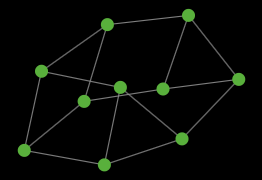
\includegraphics[width=0.8\linewidth]{../Figures/financialContagion1.png}
  \caption{\label{fig:fincont1} Initial graph with 10 agents.}
\end{subfigure}
\quad
\begin{subfigure}{.46\textwidth}
  \centering
  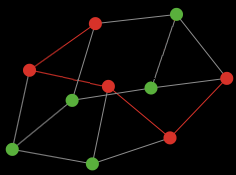
\includegraphics[width=0.8\linewidth]{../Figures/financialContagion2.png}
  \caption{\label{fig:fincont2} Insured agents (red) forms a network}
\end{subfigure}
\caption{\label{fig:fincont} shows how insured agents connects with each other to form a network to achieve super-critical payoffs.}
\end{figure}

In this model the network formation is done endogenously, and when we set up the parameters such that only insured nodes will connect, we end up with an insurable network topology. 
In this model we have neglected the information problem, we assume that all nodes can differentiate insured versus non insured nodes. This could be difficult to realize in many real world network, but in financial transactions and in software development networks, it is reasonable to assume that the parties can acquire this type of information regarding their transactional partners.

It is also possible to solve the information asymmetry problem by including a rule, such that no insured node will connect to anyone unless they can provide proof of insurance. This simple rule makes insurable-clustered components  evolve endogenously in the network. Which is beneficial for both the insurer and the nodes, because the nodes can thus receive a super-critical payoff, and they are also insured against contagious risk.  

Figure \ref{fig:GTmodel1equations} presents the individual payoffs in a formation game between two agents in the described model. It is assumed that both agents has to have a desire to establish a connection in order to create a link between them. This is reasonable since a company would not prefer to enter into an agreement with negative expected payoff. As in this case would be the result when an insured agent is requested a connection with someone without insurance. 
 
 
\begin{figure}[h]
\centering
\begin{tabular}{@{}c@{}}
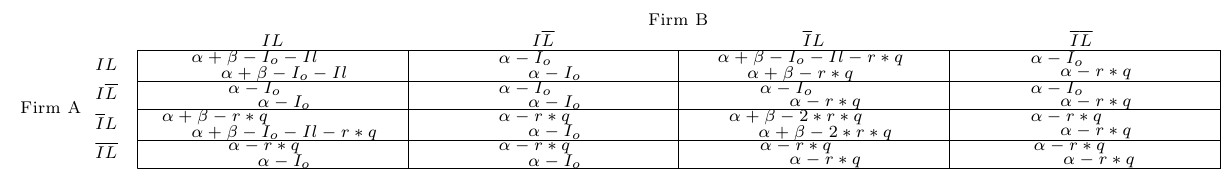
\includegraphics[width=1.0\textwidth]{../Figures/gameTheoryModel1WithEquations.png}
\end{tabular}
\caption[Caption for LOF]{\label{fig:GTmodel1equations} Normal form game between two agents individually choosing to purchase insurance and express desire to connect to the other  \footnotemark }
\end{figure}
\footnotetext{A link will only be created if both agents wishes to establish a connection.}

If we give value to the variables in figure \ref{fig:GTmodel1equations} one can observe the model's different equilibrium's. It is difficult to know exactly how the variables are set and this would vary considerably between different markets. In a real worlds scenario the variables would also be different for each agent. However in figure \ref{fig:GTmodel1} we decided to set a fixed value (which is assumed to be corresponding to the real values) for each variable in order to show a concept of how cyber-insurance can be used to create beneficial payoffs.
The following values where used: $\alpha$ = 10, $\beta$ = 10, $I_{o}$ = 5, $I_{l}$ = 2, $r$  = 20, $q$ = 0.5.


\begin{figure}[h]
\centering
\begin{tabular}{@{}c@{}}
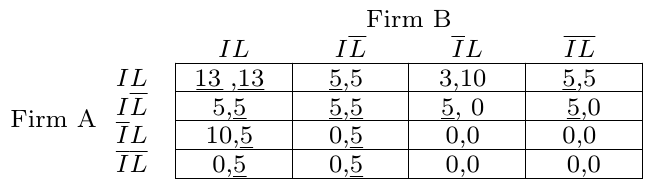
\includegraphics[width=0.6\textwidth]{../Figures/gameTheoryModel1WithNumbers.png}
\end{tabular}
\caption{\label{fig:GTmodel1} Shows equilibrium's in the resulting payoff matrix.}
\end{figure}

From the payoff matrix \ref{fig:GTmodel1} we observe two different Nash equilibrium's: One when both agents are insured and wants to connect to the other agent, and one when both are insured but does not want to establish a connection. These are the possible outcomes between the two agents, however as we can see it the social optimal solution would be for two insured agents to connect with each other, i.e they would both receive a significantly higher payoff. This demonstrates that a cluster of insured nodes would achieve higher payoffs.  
